\documentclass[../../main.tex]{subfiles}

\begin{document}

\setchapterpreamble[u]{\margintoc}

\chapter{树}

树是一个十分重要的数据结构,尤其以二叉树为例。本章主要记录如何解决一些树相关的问题。

\section{二叉树的遍历}

二叉树的遍历是一个十分重要的问题,我们可以使用递归的方式来解决这个问题,但是递归的方式十分的简单,本节
主要介绍使用非递归的方式实现二叉树的遍历。

\subsection{\href{https://leetcode.cn/problems/binary-tree-preorder-traversal/}
{二叉树的前序遍历}}

我们举一个简单的例子,来说明如何使用迭代的方式实现二叉树的前序遍历。如下图所示,我们首先需要访问
根节点5,然后需要访问其左节点。这就来到了问题的关键地方,我们必须保存节点5,以便在遍历完其左孩子,
能够访问其右孩子。对于每一个节点,我们都这样操作\sidenote{在此处,我忽略了细节的操作,实际上我认为
我们掌握这个思维方式才是最重要的,这样我们就能写出循环了,因为每一个节点都是这样的。}。

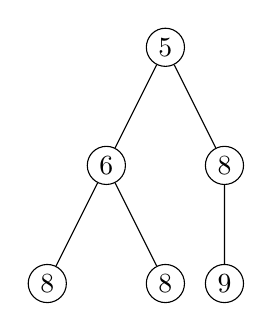
\begin{tikzpicture}[every node/.style={draw, circle, inner sep=2pt}]
  \node {5}
    child {node {6}
      child {node {8}}
      child {node {8}}
    }
    child {node {8}
      child {node {9}}
    };
\end{tikzpicture}

这样,我们就可以写出如下的代码:

\lstinputlisting[language=C++]{code/binary-tree-preorder-traversal.cpp}

\subsection{\href{https://leetcode.cn/problems/binary-tree-inorder-traversal/}
{二叉树的中序遍历}}

当我们写出了二叉树的前序遍历,我们就能写出二叉树的中序遍历了。我们只需要将前序遍历的代码稍作修改即可。
我们需要将节点保存在栈中,当我们访问完左孩子后,再访问中间节点。

\lstinputlisting[language=C++]{code/binary-tree-inorder-traversal.cpp}

\subsection{\href{https://leetcode.cn/problems/binary-tree-postorder-traversal/}
{二叉树的后序遍历}}

二叉树的后序遍历是使用迭代方法最难写的一个算法。因为我们必须在最后访问根节点,但是我们并不知道何时
这个节点的右子树已经遍历完成了,所以我们可以使用一个变量\texttt{pre}来保存上一次访问的节点,如果
当前节点的右子树已经遍历完成了,那么我们就可以访问当前节点了。即\texttt{ptr->right == pre}。
通过这个小技巧,我们就可以得出二叉树的后序遍历的非递归算法了。

\begin{kaobox}[title=二叉树统一迭代遍历方法]
  通过上述的三个代码,我们已经总结出了二叉树统一迭代遍历的方法。Amazing。
\end{kaobox}

\lstinputlisting[language=C++]{code/binary-tree-postorder-traversal.cpp}

\subsection{\href{https://leetcode-cn.com/problems/binary-tree-level-order-traversal/}
{二叉树的层序遍历}}

二叉树的层序遍历是典型的广度优先搜索算法,通过一个队列保存每层的节点即可,直到队列为空。

\lstinputlisting[language=C++]{code/binary-tree-level-order-traversal.cpp}

当解决了这个问题,我们可以解决如下的问题,其本质都是同一个思路:

\begin{itemize}
  \item \href{https://leetcode-cn.com/problems/binary-tree-zigzag-level-order-traversal/}
  {二叉树的锯齿形层序遍历}
  \item \href{https://leetcode.cn/problems/binary-tree-level-order-traversal-ii}
  {二叉树的层序遍历 II}
  \item \href{https://leetcode.cn/problems/average-of-levels-in-binary-tree}
  {二叉树的层平均值}
  \item \href{https://leetcode.cn/problems/n-ary-tree-level-order-traversal}
  {N叉树的层序遍历}
\end{itemize}

\section{二叉树的构建}

\subsection{\href{https://leetcode-cn.com/problems/construct-binary-tree-from-preorder-and-inorder-traversal/}
{从前序与中序遍历序列构造二叉树}}

要解决这个问题,我们首先需要思考前序遍历和中序遍历的特点。前序遍历的第一个节点一定是根节点,而中序遍历
的根节点左边的节点都是左子树的节点,右边的节点都是右子树的节点。因此,我们可以通过前序遍历的第一个节点
来确定根节点,然后在中序遍历中找到根节点的位置,然后递归地处理左子树和右子树。

然而,最关键的问题在于,我们应该先处理左子树还是右子树,这个问题的答案是,我们应该先处理左子树。因为
我们在前序遍历中,先访问的是根节点,然后是左子树,最后是右子树。因此,我们应该先处理左子树,然后再处理
右子树。为了快速地找到根节点在中序遍历中的位置,我们可以使用一个哈希表来存储中序遍历中每个节点的位置。

\lstinputlisting[language=C++]
{code/construct-binary-tree-from-preorder-and-inorder-traversal.cpp}

\subsection{\href{https://leetcode-cn.com/problems/construct-binary-tree-from-inorder-and-postorder-traversal/}
{从中序与后序遍历序列构造二叉树}}

这个问题和上一个问题的思路是一样的,只不过我们需要先处理右子树,然后再处理左子树。

\lstinputlisting[language=C++]{code/construct-binary-tree-from-inorder-and-postorder-traversal.cpp}

\subsection{\href{https://leetcode-cn.com/problems/construct-binary-tree-from-preorder-and-postorder-traversal/}
{根据前序和后序遍历构造二叉树}}

实际上前序遍历和后序遍历并不能唯一确定一棵二叉树,因为我们无法确定左子树和右子树的边界。但是,这个问题只需要
我们还原出任意一个符合条件的二叉树即可。

我们可以采取一个十分简单的思路。取当前节点的前序遍历的下一个节点作为其左子树的根节点,然后在后序遍历中确定该节点
的前一个节点作为其右子树的根节点。这样,我们就可以递归地构建出一棵二叉树了。但是这样我们还需要做一个工作,就是需要
记录这个节点是否已经被使用过了,如果使用过了,我们就不能再使用了。这个思路实际上并不能算上很优雅,但是这个解法
很直观且简单\sidenote{实际上,这个题确实是有更加优雅的做法。既然我们能够确定出当前节点的左子树的根节点以及其右子树
的根节点,那么我们就能够用长度的方式代替我们使用的\texttt{visited}变量,但我个人认为我这个思路是容易理解的。}。

\lstinputlisting[language=C++]{code/construct-binary-tree-from-preorder-and-postorder-traversal.cpp}

\section{二叉树的基础题目}

\subsection{\href{https://leetcode.cn/problems/maximum-depth-of-binary-tree/}{二叉树的最大深度}}

这个题我们只需要简单地使用递归进行处理即可,对于空节点,我们返回0,对于非空节点,我们返回左右子树的最大深度加1。
显然,利用二叉树的前序遍历我们就可以简单地得出如下的代码:

\lstinputlisting[language=C++]{code/maximum-depth-of-binary-tree.cpp}

\subsection{\href{https://leetcode-cn.com/problems/minimum-depth-of-binary-tree/}{二叉树的最小深度}}

似乎我们可以直接调用上一题的代码,把 。然而这样是不行的。因为如果我们的二叉树只有左子树或者只有右子树,那么我们的代码
会返回0,但是实际上这个二叉树的最小深度是3。如下图所示:

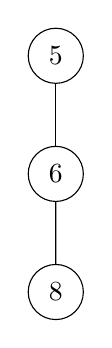
\begin{tikzpicture}[every node/.style={circle,draw,minimum size=7mm}]
  \node (5) {5}
    child {node (6) {6}
      child {node (8) {8}}};
\end{tikzpicture}

因此,当有某个节点其左子树或者右子树为空时,我们会得到其深度为0。当遇到了这样的情况,我们应该返回左子树
和右子树的最大的深度加1。当不会出现这样的情况时,我们就可以返回左子树和右子树的最小深度加1了。于是,我们
就可以得出如下的代码:

\lstinputlisting[language=C++]{code/minimum-depth-of-binary-tree.cpp}


\end{document}
